At $\kappa=2$ the retained block holds 97.9\% of the energy of a volume but only 33\% of a voxel's temporal variance (Fig.~\ref{fig:oracle}). The relaxation lowers the voxel error because it keeps the static anatomy, and for the same reason it cannot express two thirds of the dynamics that an EEG could inform.

\begin{figure}[ht]
	\centering
	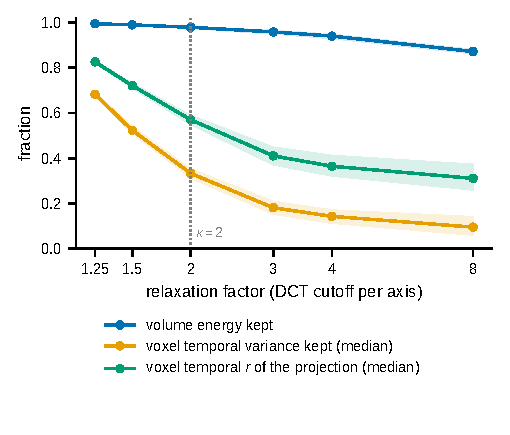
\includegraphics[width=0.55\textwidth]{figures/oracle_bound.pdf}
	\caption{Oracle projection onto the retained DCT block: the volume energy is almost entirely kept, but most of each voxel's temporal variance is not. Lines: mean over subjects; bands: range over subjects.}
	\label{fig:oracle}
\end{figure}

\begin{table}[!htbp]
	\centering
	\caption{UQ benchmark on CHUR-XP2, run-z-score target (17 test subjects; seeds averaged). Lower is better for RMSE ($\pm$ SD over seeds), NLL, CRPS and AUSE. PICP$_{90}$: coverage of the model's own 90\% interval; Conf$_{90}$: of the per-voxel split-conformal 90\% interval; $\rho$: Spearman correlation between predictive SD and absolute error. Last three columns: one-sided paired Wilcoxon $p$ for NLL below the population template, and median voxel $r$ above the shift and swap nulls (bold: $p<0.05$). The own-subject oracle uses test data. $^\dagger$Diverged in every seed.}
	\label{tab:uq}
	\setlength{\tabcolsep}{3pt}
	\resizebox{\textwidth}{!}{%
	\begin{tabular}{lcccccccccc}
		\toprule
		Method & RMSE & NLL & CRPS & PICP$_{90}$ & Conf$_{90}$ & $\rho$ & AUSE & $p_{\mathrm{NLL}<\mathrm{tmpl}}$ & $p_{r>\mathrm{shift}}$ & $p_{r>\mathrm{swap}}$\\
		\tabinput{tables/uq_benchmark}
		\bottomrule
	\end{tabular}}
\end{table}

The population template, which never sees EEG, has an NLL of 0.463, a CRPS of 0.239 and an RMSE of 0.520 (Table~\ref{tab:uq}). Our results show that no method is significantly better on any of the three. The deep ensemble comes closest (NLL 0.393, $p=0.23$), mostly through mixing: its members average 0.522. For every single-model method an NLL gain of at least the smallest effect of interest is rejected (Supplementary Table~S1).

\begin{figure}[!htbp]
	\centering
	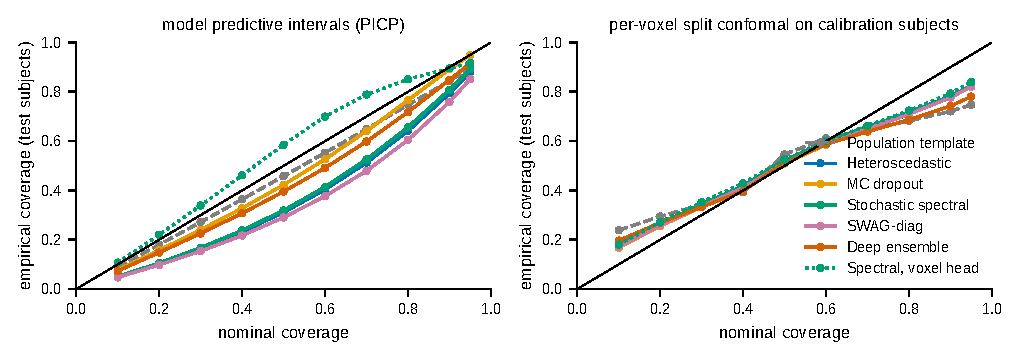
\includegraphics[width=\textwidth]{figures/reliability.pdf}
	\caption{Reliability on test subjects (run-z-score target). Left: coverage of each model's own central intervals. Right: after per-voxel split conformal calibration on two held-out subjects. The EEG-free template (dashed) is as well calibrated as any network.}
	\label{fig:reliability}
\end{figure}
The usual diagnostics do not separate the networks from the template either (Fig.~\ref{fig:reliability}): the template is as well calibrated, and its spread tracks its error better ($\rho=0.52$ vs 0.47--0.51). After conformal calibration on two subjects every method, the template included, under-covers (72--79\% at 90\%); calibrating on all 16 other subjects restores 88--90\% (Supplementary Table~S6).

\textbf{Predicted uncertainty does not depend on the EEG}\label{sec:res:nulls}
\begin{figure}[!htbp]
	\centering
	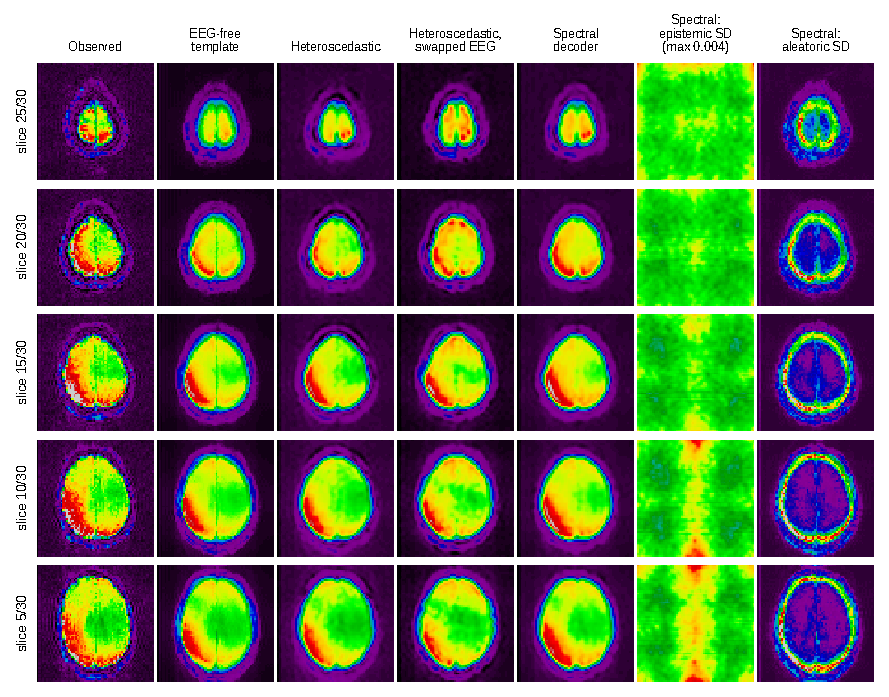
\includegraphics[width=\textwidth]{figures/volumes.pdf}
	\caption{Synthesized volumes for one CHUR-XP2 test subject (first test volume, fold 0, seed 2). From left: the observed volume; the EEG-free population template; the heteroscedastic network with the subject's EEG and with another subject's EEG; the stochastic spectral decoder's prediction, and its epistemic and aleatoric predictive SD (own colour scales). The predictions reproduce the template whatever EEG is given, and the aleatoric SD follows the anatomy. The epistemic SD is a mirror-symmetric pattern set by the DCT basis (Section~\ref{sec:res:nulls}).}
	\label{fig:volumes}
\end{figure}
No method's temporal correlation exceeds the subject-swap null, and an EEG-specific gain of $\delta_r=0.05$ is rejected for every method ($p<0.001$). All are below $r=0.016$, against 0.160 for the stimulus-locked template. The predictive spread is a fixed map (Fig.~\ref{fig:volumes}): its variance over time is $10^{-6}$ to $10^{-3}$ of its variance across voxels, the SD maps under the real, shifted and swapped EEG correlate at $1.000$, and the spread tracks the anatomical part of the error ($\rho\approx0.5$), not its temporal part (Supplementary Table~S2).

The epistemic map of the stochastic spectral decoder has no anatomy for a structural reason. Its noise enters as independent DCT coefficients $Z_k$, so its epistemic variance at voxel $v$ is $\sum_k \mathrm{Var}[Z_k]\,\phi_k(v)^2$; each squared basis function $\phi_k^2$ is unchanged by reflecting $v$ about the centre of the field of view, so the map is mirror-symmetric whatever variances are learned. Anatomy could enter only through the gains on the retained coefficients, which shrank in training (epistemic variance $4\times10^{-6}$, aleatoric 0.26). In Fig.~\ref{fig:volumes}, 73\% of the map's spatial variance is mirror-symmetric and the rest is within the Monte Carlo error of 50 samples: noise in a global basis gives global, symmetric uncertainty.

\begin{table}[!htbp]
	\centering
	\caption{Positive control: median voxel $r$ in the injected box, mean over 17 test subjects, shift and swap nulls in brackets. Ceiling: $\sqrt{s/(1+s)}$. Ridge: kernel ridge on band power of the input window. Linear and MLP: the same features with the deep models' loop (Laplace likelihood, Adam at $2.98\times10^{-3}$, batch 4, 10 epochs) or a regression loop (MSE, batch 64, 50 epochs). Backbone: heteroscedastic head, point $L_1$ loss, and heteroscedastic head at learning rate $10^{-4}$. --: not run.}
	\label{tab:positive}
	\setlength{\tabcolsep}{3pt}
	\resizebox{\textwidth}{!}{%
	\begin{tabular}{cccccccccc}
		\toprule
		$s$ & ceiling & ridge & linear, deep loop & linear, MSE & MLP, deep loop & MLP, MSE & backbone, hetero. & backbone, $L_1$ & backbone, hetero., lr $10^{-4}$\\
		\midrule
		\tabinput{tables/positive_control}
		\bottomrule
	\end{tabular}}
\end{table}
The linear probe recovers the injected signal at every strength ($r=0.59$ at $s=1$, ceiling 0.71; nulls near zero), while the heteroscedastic backbone, the base of most UQ methods, recovers it at none (Table~\ref{tab:positive}). The same backbone recovers it with a point loss ($r=0.48$) or a lower learning rate ($0.49$), and a linear map and an MLP lose it when trained with the deep models' loop: at the searched learning rate the learned variance absorbs the residual and the mean stops fitting \citep{seitzer2022pitfalls}.

\begin{figure}[!htbp]
	\centering
	\begin{subfigure}[t]{\textwidth}
		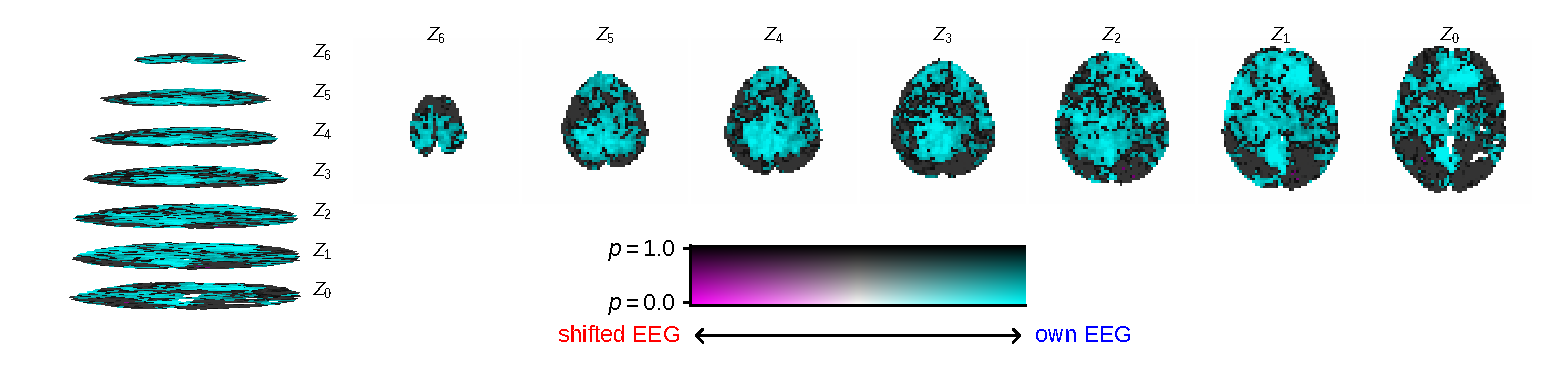
\includegraphics[width=\textwidth]{figures/sig_mni_hetero_lr1e-4_b32_fluct_real_vs_shift.pdf}
		\caption{Own EEG vs EEG shifted in time.}
	\end{subfigure}
	\begin{subfigure}[t]{\textwidth}
		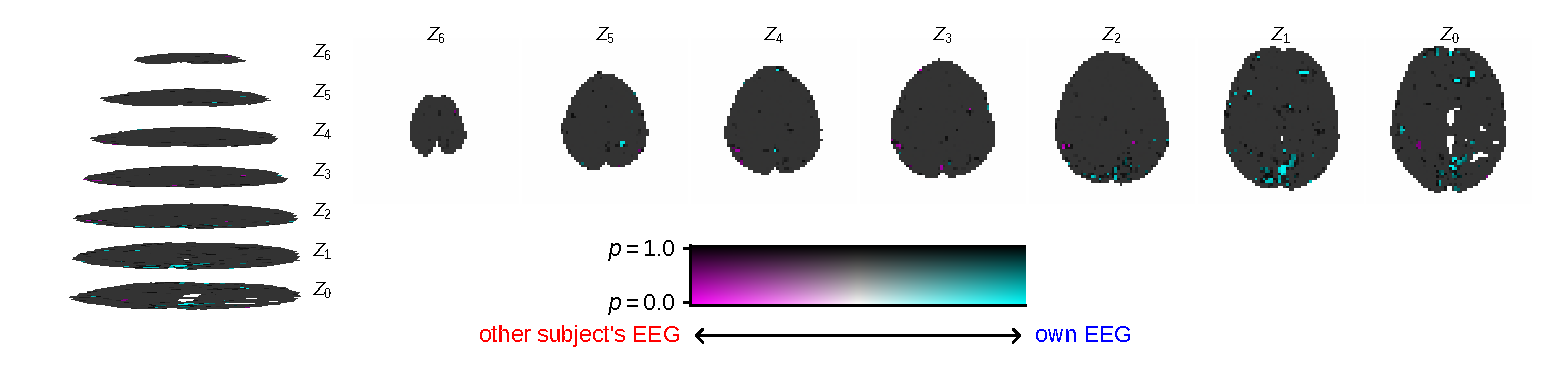
\includegraphics[width=\textwidth]{figures/sig_mni_hetero_lr1e-4_b32_fluct_real_vs_swap.pdf}
		\caption{Own EEG vs another subject's EEG.}
	\end{subfigure}
	\begin{subfigure}[t]{\textwidth}
		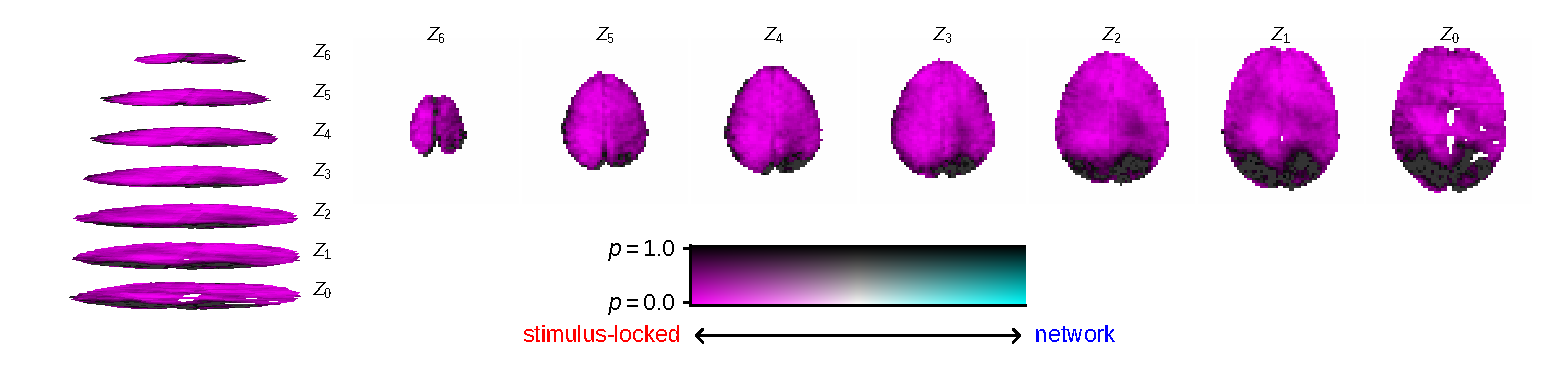
\includegraphics[width=\textwidth]{figures/sig_mni_hetero_fluct_vs_locked.pdf}
		\caption{Network vs EEG-free stimulus-locked template.}
	\end{subfigure}
	\caption{Where does the EEG help? Voxelwise paired Wilcoxon tests over the 17 CHUR-XP2 subjects of the temporal correlation between predicted and observed fluctuations, registered volumes; 13{,}785 brain voxels (mean registered EPI above half its range, all tested). Seven axial slices from the lowest slice fully inside the oblique acquisition slab ($Z_0$) to near the vertex ($Z_6$), 3-D stack at left. Grey: $p\ge0.05$; coloured: the condition named at that end of the colour bar is significantly better, brighter for larger $r$. (a, b) The heteroscedastic network at the lower learning rate, which recovers an injected signal: its own EEG beats the shifted EEG in 50\% of the voxels (cyan), but differs from another subject's EEG in 1.6\% (187 better, 30 worse), fewer than expected by chance. (c) The stimulus-locked template beats the network in 90\% of the voxels (magenta).}
	\label{fig:sigmaps}
\end{figure}
Trained with the recipes that recover the injected signal, the networks on the real fluctuations exceed the time-shift null ($r=0.030$--$0.066$, $p\le0.022$) but not the subject-swap null ($p\ge0.37$), and so does the linear probe (Fig.~\ref{fig:sigmaps}). The stimulus-locked template, which only knows when the imagery blocks occur, beats them almost everywhere. A network given only the ECG lead scores about as well as one given the EEG, and removing the task-locked response leaves nothing predictable (Supplementary Section~S4).


\begin{figure}[!htbp]
	\centering
	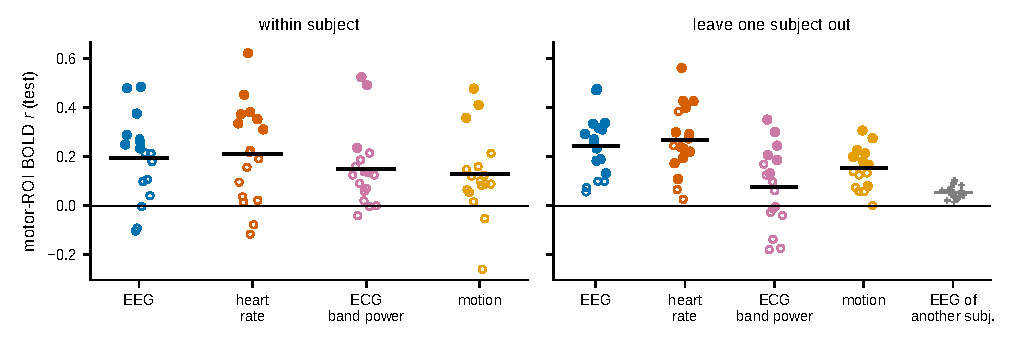
\includegraphics[width=\textwidth]{figures/ridge.pdf}
	\caption{ROI ridge across subjects, task regressed out: test correlation per subject for EEG, heart rate, ECG band power and head motion (filled: above the subject's IAAFT surrogates at $p<0.05$), and the EEG model scored on another subject's EEG. Black bars: means.}
	\label{fig:ridge}
\end{figure}
\begin{table}[!htbp]
	\centering
	\caption{Nested models: does the EEG add to the physiological confounds? Held-out $R^2$ of the confounds alone and with the EEG, task regressed out; $\Delta R^2$ with the one-sided Wilcoxon $p$ of a gain, and $\Delta R^2$ with another subject's EEG.}
	\label{tab:nested}
	\small
	\begin{tabular}{llcccccc}
		\toprule
		Design & confounds & $n$ & $R^2$ reduced & $R^2$ full & $\Delta R^2$ & $p_{\Delta>0}$ & $\Delta R^2$ swap\\
		\midrule
		\tabinput{tables/ridge_nested}
		\bottomrule
	\end{tabular}
\end{table}
\textbf{At the region level, heart rate predicts as much as the EEG.} Within subjects the EEG and heart-rate ridges each beat their surrogates in 7 of 17 subjects, but no model beats the block design. Across subjects the EEG ridge looks like a success: with the task regressed out it reaches $r=0.243$, 13 of 17 subjects beat their surrogates (binomial $p<0.001$), and it beats the swap null ($p<0.001$; Fig.~\ref{fig:ridge}), although not the block design ($p=0.066$). But heart rate alone predicts the same region as well ($r=0.268$, 13 of 17; EEG not better, $p=\ridgeEEGvsHR$), and in nested models the EEG adds nothing to heart rate and motion across subjects ($\Delta R^2=-0.001$, $p=0.50$; Table~\ref{tab:nested}). Within subjects it adds a small amount ($\Delta R^2=0.028$, $p=0.044$, uncorrected) that does not survive adding the ECG band power to the confounds ($\Delta R^2=0.013$, $p=0.15$). The EEG also still carries the heart: after pulse-artefact correction, 20\% of its band-power features correlate with heart rate at $|r|>0.2$, against 1.7\% with a shifted heart rate ($p<0.001$).

The pipeline and test of \citet{mehta2025eegbold}, applied as published, also support EEG-to-BOLD prediction here (trial-evoked $r=0.182$ within runs, 8 of 16 subjects beyond surrogates, binomial $p<0.001$, better than both of their reference models, FDR-corrected $p=0.005$), and the same pipeline on the ECG lead alone does nearly as well ($r=0.149$, 9 of 16; Supplementary Table~S10).

\subsection{Replication on CHUR-XP1}\label{sec:res:xp1}
On CHUR-XP1 the voxel-level results and the positive control replicate (Supplementary Table~S4). No model exceeds the swap null, the predicted SD maps under real and null EEG correlate at 1.000, and the point-loss backbone recovers the injected signal ($r=0.37$) while the heteroscedastic one does not ($r=-0.02$). Two methods have a lower NLL than the template (ensemble $p=0.004$, stochastic spectral decoder $p=0.020$) but none a lower CRPS or RMSE, which we read as a calibration effect of six or seven training subjects. At the region level the EEG ridge again predicts the ROI across subjects ($r=0.172$, 7 of 9), heart rate nearly as well ($r=0.137$; EEG not better, $p=0.18$), and the EEG adds nothing to heart rate and motion ($\Delta R^2=-0.005$, $p=0.54$).
